\documentclass{exam}
%\documentclass[answers]{exam}
\hbadness=99999
\usepackage[total={6.5in,9in}]{geometry}

\usepackage{enumerate}
\usepackage{amsmath}
\usepackage[table]{xcolor}
\usepackage{graphicx}
\usepackage{tikz}
\usetikzlibrary{shapes.multipart}
%\usepackage{pgfplots}
\usepackage{multicol}

% for syntax highlighting
\usepackage{minted}
\usemintedstyle[cpp]{xcode}

% for overlay of output
\usepackage[overlay,showboxes]{textpos}

\pagestyle{plain}

\setlength\columnsep{50pt}
\newcommand{\key}{\hfill
      \raisebox{-.3\height}{\includegraphics[width=0.6in]{figures/key.png}}}

\begin{document}
  \thispagestyle{empty}
  \setlength{\parindent}{0pt}

  \begin{center}
    \Large Activity \#8: Recursion \\[5pt]
    \large Recorder's Report\\[20pt]
    \normalsize
    \begin{tabular}{lrp{0.1in}lr}
      Manager:  & \fillin[][2.0in] & & Presenter: & \fillin[][2.0in]\\[15pt]
      Recorder: & \fillin[][2.0in] & & Driver:    & \fillin[][2.0in]\\[15pt]
      Date:     & \fillin[][2.0in] & & Score:     & Satisfactory \hspace{10pt} /
      \hspace{10pt} Not Satisfactory
    \end{tabular}
  \end{center}
  \par\vskip 15pt
  
  Record your group's answers to the key questions (marked with
  \raisebox{-.3\height}{\includegraphics[width=0.5in]{figures/key.png}})
  below.
  \begin{enumerate}[(a)]
    \itemsep 1.75in
    \item Model 1, Question \#2
    \item Model 2, Question \#7
    \item Model 3, Question \#17
  \end{enumerate}

  \clearpage\pagenumbering{arabic} 
  
  \begin{center}
    \Large Activity \#8: Recursion \\[5pt]
    \large Activity Guide\\[20pt]
  \end{center}

  \begin{center}
    \fbox{
      \begin{minipage}{5.5in}
        {\bf Learning Objectives:} Students will be able to:
        \begin{itemize}
          \item Content:\\[-20pt]
            \begin{itemize}           
              \itemsep 0pt
              \item Identify the base case and recursive step of the
                factorial function
              \item Trace a recursive function by hand and and predict its
                final output
              \item Explain what happens in memory when a function
                calls itself
            \end{itemize}
          \item Process\\[-20pt]
            \begin{itemize}
              \itemsep 0pt
              \item Write a recursive function to compute the sum of
                the first $n$ numbers\\[-5pt]
            \end{itemize}
        \end{itemize}
      \end{minipage}
      }
  \end{center}
  \par\vskip 10pt
  
  
  {\bf\large Model 1: The Factorial Function}\\
  \begin{center}
    \renewcommand{\arraystretch}{1.2}
    \begin{tabular}{c|cccccc}
      $n$ & 0 & 1 & 2 & 3 & 4 & 5 \\
      \hline
      $n!$ & 1 & 1 & 2 & 6 & 24 & 120 \\
    \end{tabular}
  \end{center}
  \par\vskip 5pt
  
  {\it\large Refer to Model 1 above as your group develops consensus answers
    to the questions below.}
    \par\vskip 10pt
    
  \begin{enumerate}
    \itemsep 20pt
    
    \item In mathematics, the {\it factorial} function for a natural
      number $n$ is denoted by $n!$.  It is the product of all positive
      integers less than or equal to $n$.  For example:
      \[
        5! = 5\times 4 \times 3 \times 2 \times 1 = 120
      \]
      Consider how to calculate $4!$.
      \par\vskip 10pt
      \begin{enumerate}
        \item Write out all of the numbers that need to be multiplied
          to get $4!$.
          \begin{solution}[0.5in]
            \[ 4! = 4\times 3\times 2\times 1 \]
          \end{solution}
        \item Rewrite the expression using $3!$ instead of $3\times
          2\times 1$.
          \begin{solution}[0.5in]
            \[ 4! = 4\times 3! \]            
          \end{solution}
      \end{enumerate}
      \par\vskip -40pt\null
      
    \item Express the factorials as a product of a single
      natural number with a simpler factorial\key\\[-2mm].
      \par\vskip 15pt
      \begin{enumerate}
        \itemsep 15pt
        \begin{multicols}{2}
          \item $3! =$ \hfill \fillin[$3 \times 2!$][2in]
          \item $2! =$ \hfill \fillin[$2 \times 1!$][2in]
          \item $100! = $\hfill \fillin[$100 \times 99!$][2in]
          \item $n! = $\hfill \fillin[$n\times (n-1)!$][2in]
        \end{multicols}
      \end{enumerate}
      
    \item Now consider the very first natural number, 0.
      \par\vskip 10pt
      \begin{enumerate}[(a)]
        \item Based on the model, what is the value of
          $0!$? \fillin[1][1.5in]\par\vskip 10pt
        \item Does it make sense to define $0!$ in terms of a simpler
          factorial?  Explain.        
          \begin{solution}[0.5in]
            No, we can't say that $0 \times -1! = 1$ because factorial
            is only defined for non-negative numbers.
          \end{solution}
        \item When we define the value of a function by
          referencing that same function for a simpler value, we will
          eventually reach a point where there are no simpler values
          and we have to just give a concrete value to the function.
          This is called a {\it base case}.  What is the base case for
          the factorial function?
          \begin{solution}[0.5in]
            The base case is $0! = 1$.
          \end{solution}
      \end{enumerate}
      
    \item Suppose you already have a working implementation of the
      function declared below.
      \begin{center}
        \mintinline{cpp}|int factorial(int n);|
      \end{center}
      \par\vskip 5pt
      \begin{enumerate}
        \itemsep 15pt
        \item How could you compute $100!$ without calling
          \mintinline{cpp}|factorial(100)|?  Give a C++ command to do this.
          \begin{solution}[0.5in]
          \end{solution}
        \item How could you compute $n!$ without calling
          \mintinline{cpp}|factorial(n)|?  Give a C++ command to do this.
          \begin{solution}[0.5in]
          \end{solution}
      \end{enumerate}
      \par\vskip 10pt


  {\bf\large Model 2: A C++ Factorial Function}\\[-20pt]
  
    \begin{center}
      \begin{minipage}{5in}
        \begin{minted}[
          frame=lines,
          framesep=2mm,
          bgcolor=gray!15,
          baselinestretch=1.2,
          linenos,
          firstnumber=4
        ]{cpp}
int factorial(int n) {
  cout << "n is " << n << endl;
  if (n == 0) {
    return 1;    // base case
  } else {
    cout << "need factorial of " << (n-1) << endl;
    int answer = factorial(n-1);
    cout << "factorial of " << (n-1) << " is " << answer << endl;
    return n * answer;
  }
}
        \end{minted}      
      \end{minipage}
    \end{center}

  {\it\large Refer to Model 2 above as your group develops consensus answers
    to the questions below.}
  \par\vskip 10pt
  
    \item This model gives a definition of the
      \mintinline{cpp}|factorial| function.  Use it to answer the
      following questions.
      \par\vskip 15pt
      \begin{enumerate}
        \itemsep 15pt
        \item What specific function is called on line 10?
          \hfill\fillin[][2.5in]
        \item Why is the \mintinline{cpp}|if| statement on line 6
          needed?
          \begin{solution}[0.5in]
          \end{solution}       
      \end{enumerate}
      
    \item A function that calls itself is called {\it recursive}.
      What two steps are required to define the recursive function
      \mintinline{cpp}|factorial|?
      \begin{solution}[0.75in]
      \end{solution}
      \par\vskip -30pt\null
      
    \item Because recursive functions call themselves as a part of
      their execution, it takes some\key\\[-2.5mm] thought to understand 
      their execution.
      \begin{enumerate}[(a)]
        \itemsep 15pt
        \item How many distinct function calls would be made to the
          \mintinline{cpp}|factorial| function to compute $2!$?
          Identify the function argument for each of those calls.
          \begin{solution}[0.5in]
          \end{solution}
        \item How many distinct function calls would be made to the 
          \mintinline{cpp}|factorial| function to compute $4!$?
          Identify the function argument for each of those calls.
          \begin{solution}[0.5in]
          \end{solution}
      \end{enumerate}
      
    \item The file {\tt activity08.cpp} contains the function from    
      this model along with a test function call to compute $5!$.  Run
      this program and then identify the function call which produces
      each line of output below.  Several have been done for you.
      \par\vskip 15pt
      
      \begin{enumerate}
        \itemsep 15pt
        \begin{multicols}{2}
          \item {\tt n is 5} \hfill\underline{\tt\hspace{4pt}factorial(5)\hspace{4pt}}
          \item {\tt need factorial of 4} \hfill\fillin[][1in]
          \item {\tt n is 4} \hfill\fillin[][1in]
          \item {\tt need factorial of 3} \hfill\fillin[][1in]
          \item {\tt n is 3} \hfill\fillin[][1in]
          \item {\tt need factorial of 2} \hfill\fillin[][1in]
          \item {\tt n is 2} \hfill\fillin[][1in]
          \item {\tt need factorial of 1} \hfill\underline{\tt\hspace{5pt}factorial(2)\hspace{5pt}}
          \item {\tt n is 1} \hfill\fillin[][1in]
          \item {\tt need factorial of 0} \hfill\fillin[][1in]
          \item {\tt n is 0} \hfill\fillin[][1in]
          \item {\tt factorial of 0 is 1} \hfill\underline{\tt\hspace{5pt}factorial(1)\hspace{5pt}}
          \item {\tt factorial of 1 is 1} \hfill\fillin[][1in]
          \item {\tt factorial of 2 is 2} \hfill\fillin[][1in]
          \item {\tt factorial of 3 is 6} \hfill\fillin[][1in]
          \item {\tt factorial of 4 is 24} \hfill\fillin[][1in]
        \end{multicols}
      \end{enumerate}
      
    \item What happens if you try to calculate the factorial of a
      negative number?  Explain why this happens.
      \begin{solution}[0.75in]
      \end{solution}
      
    \item How could you prevent this behavior?
      \begin{solution}[0.75in]
      \end{solution}

    \item What is the largest factorial you can compute in C++ without
      changing the types of the variables in this function?  Play with
      the code in {\tt activity08.cpp} to find out.
      \begin{solution}[0.75in]
      \end{solution}
      
      
  {\bf\large Model 3: Summations}\\[-30pt]
  \begin{center}
    \[
      \sum_{i=1}^{100} i = 1 + 2 + 3 + \cdots + 100 = 5050
    \]
  \end{center}
  
  {\it\large Refer to Model 3 above as your group develops consensus answers
    to the questions below.}
  \par\vskip 10pt
    
  \item In mathematics, {\it summation} (represented by the Greek
    letter ``sigma'', $\Sigma$) is the addition of a sequence of
    numbers resulting in a single sum or total. For example, 
    \[
      \sum_{i=1}^{i=3} i = 1 + 2 + 3 = 6
    \]
    Consider how to calculate $\displaystyle \sum_{i=1}^{5} i$.
    \par\vskip 15pt
    \begin{enumerate}[(a)]
      \itemsep 15pt
      \item Write out all the numbers that need to be added.
        \begin{solution}[0.5in]
        \end{solution}
      \item Show how this sum can be calculated in terms of a smaller
        summation.
        \begin{solution}[0.5in]
        \end{solution}
    \end{enumerate}
      
  \item Express the summations as a sum of a single
    natural number and a shorter summation.
    \par\vskip 15pt
    \begin{enumerate}
      \itemsep 15pt
      \begin{multicols}{2}
        \item $\displaystyle \sum_{i=1}^{100} i = $ \hfill \fillin[][2in]
        \item $\displaystyle \sum_{i=1}^n i = $ \hfill \fillin[][2in]
      \end{multicols}
    \end{enumerate}
    
  \item The base case for this summation is: \hfill\fillin[][4in]
  
  \item Write a C++ function {\tt summation} that takes a single
    parameter {\tt n} and returns the sum $1 + 2 + \cdots + n$.  It
    should only have an \mintinline{cpp}|if| statement and two 
    \mintinline{cpp}|return| statements.
    \begin{solution}[1.5in]
    \end{solution}
    \par\vskip 10pt
    
  \item Below is a different recursive implementation of the
    {\tt factorial} function seen in model 2.
    \par\vskip -20pt\null
    
    \begin{center}
      \begin{tabular}{p{2.5in}p{3.5in}}
        \begin{minipage}{2.5in}
          \begin{minted}[
            frame=lines,
            framesep=2mm,
            bgcolor=gray!15,
            baselinestretch=1.2,
            linenos,
          ]{cpp}
int factorial(int n) {
  if (n == 0) {
    return 1; // base case
  }
  int recurse = factorial(n-1);
  int result = n * recurse;
  return result;
}
          \end{minted}
        \end{minipage}
        &
        \begin{minipage}{3.5in}
          \begin{enumerate}
            \item How are temporary variables used in this function?
              \begin{solution}[0.5in]
              \end{solution}
            \item What would you change to change this to a {\tt
              summation} function?
              \begin{solution}[0.5in]
              \end{solution}              
          \end{enumerate}
        \end{minipage}
      \end{tabular}
    \end{center}
    \par\vskip 50pt
        
    \item Below is a {\it stack diagram} of a call to this implementation
      of \mintinline{cpp}|factorial(3)| from the {\tt main}\key\\[-2.5mm] program.
      Sketch a similar diagram for a call to \mintinline{cpp}|summation(3)|.
      \begin{center}
        \begin{tabular}{p{3in}p{3in}}
          \begin{minipage}{3in}
            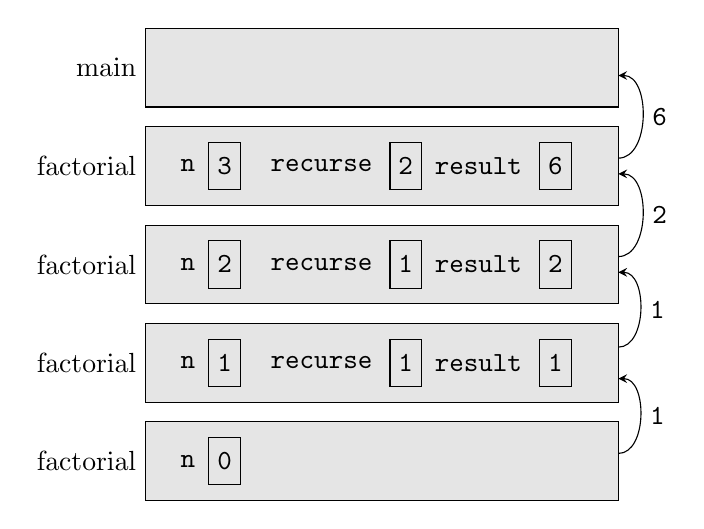
\begin{tikzpicture}
            
              \draw[fill=gray!20] (0,5) rectangle (6,6);
              \node[left] at (0,5.5) {main};

              \draw[fill=gray!20] (0,3.75) rectangle (6,4.75);
              \node[left] at (0,4.25) {factorial};
              \node[left] at (0.75,4.25) {\tt n};
              \draw (0.8,3.95) rectangle (1.2,4.55) node[pos=.5] {\tt 3};
              \node[left] at (3,4.25) {\tt recurse};
              \draw (3.1,3.95) rectangle (3.5,4.55) node[pos=.5] {\tt 2};
              \node[left] at (4.9,4.25) {\tt result};
              \draw (5,3.95) rectangle (5.4,4.55) node[pos=.5] {\tt 6};
            
              \draw[fill=gray!20] (0,2.5) rectangle (6,3.5);
              \node[left] at (0,3) {factorial};
              \node[left] at (0.75,3) {\tt n};
              \draw (0.8,2.7) rectangle (1.2,3.3) node[pos=.5] {\tt 2};
              \node[left] at (3,3) {\tt recurse};
              \draw (3.1,2.7) rectangle (3.5,3.3) node[pos=.5] {\tt 1};
              \node[left] at (4.9,3) {\tt result};
              \draw (5,2.7) rectangle (5.4,3.3) node[pos=.5] {\tt 2};
            
              \draw[fill=gray!20] (0,1.25) rectangle (6,2.25);
              \node[left] at (0,1.75) {factorial};
              \node[left] at (0.75,1.75) {\tt n};
              \draw (0.8,1.45) rectangle (1.2,2.05) node[pos=.5] {\tt 1};
              \node[left] at (3,1.75) {\tt recurse};
              \draw (3.1,1.45) rectangle (3.5,2.05) node[pos=.5] {\tt 1};
              \node[left] at (4.9,1.75) {\tt result};
              \draw (5,1.45) rectangle (5.4,2.05) node[pos=.5] {\tt 1};
            
              \draw[fill=gray!20] (0,0) rectangle (6,1);
              \node[left] at (0,0.5) {factorial};
              \node[left] at (0.75,0.5) {\tt n};
              \draw (0.8,0.2) rectangle (1.2,0.8) node[pos=.5] {\tt 0};
              
              \draw[-stealth] (6,0.6) to [out=0,in=0] node[right] {\tt 1} (6,1.55);
              \draw[-stealth] (6,1.95) to [out=0,in=0] node[right] {\tt 1} (6,2.9);
              \draw[-stealth] (6,3.1) to [out=0,in=0] node[right] {\tt 2} (6,4.15);
              \draw[-stealth] (6,4.35) to [out=0,in=0] node[right] {\tt 6} (6,5.4);
              
            \end{tikzpicture}
          \end{minipage}
          &
          \begin{minipage}{3in}
          \end{minipage}
        \end{tabular}
      \end{center}
      \newpage
        
    \item Why are there no values for {\tt recurse} and {\tt result}
      in the stack diagram for the last call to {\tt factorial} (when
      \mintinline{cpp}|n == 0|)?      
      \begin{solution}[1.5in]
      \end{solution}
      
    \item Looking at the stack diagram, how is it possible that the
      parameter {\tt n} can have multiple values in memory at the same
      time?
      \begin{solution}[1.5in]
      \end{solution}

  \end{enumerate}
  
  
    
\end{document}
